\documentclass[english,aspectratio=1610]{beamer}
\usepackage[T1]{fontenc}
\usepackage[utf8]{inputenc}
\usepackage[english]{babel}
\usepackage{graphicx}
\usepackage{caption} 
\usepackage[round]{natbib}

\usepackage{xspace}
\usepackage{xmpmulti}
\usepackage{tabularx}
\usepackage{tabto}
\usepackage{media9}
\usepackage{array}
\usepackage{multicol}
\usepackage{xcolor}
\usepackage{afterpage}
\usepackage{amsmath,amssymb}            
\usepackage{rotating}  
\usepackage{fancyhdr}  
%\usepackage[scriptsize]{caption} 
\usepackage{cite}
\usepackage{hyperref}
\usepackage{cleveref}

\usepackage{algpseudocode}
\usepackage{algorithm}
\usepackage{algorithmicx}
%%%%%%%%%%%%%%%%%%%%%%% ALGORITHM COMMAND %%%%%%%%%%%%%%%%%
\algrenewcommand\algorithmicrequire{\textbf{Input:}}
\algrenewcommand\algorithmicensure{\textbf{Output:}}

% MATH
\usepackage{amsmath,amssymb,amsthm,mathrsfs,amsfonts,dsfont}    
\usepackage{mathtools}
\usepackage{bm}
\usepackage[customcolors]{hf-tikz}

%%%%% MATH COMMANDS
\newcommand{\sas}{\int_\mathcal{S} \int_\mathcal{A} \int_\mathcal{S}}


%COLORS
\makeatletter
\newcommand{\algcolor}[2]{%
	\hskip-\ALG@thistlm\colorbox{#1}{\parbox{\dimexpr\linewidth-2\fboxsep}{\hskip\ALG@thistlm\relax #2}}%
}
\makeatother
\definecolor{aliceblue}{rgb}{0.94, 0.97, 1.0}
\definecolor{bisque}{rgb}{1.0, 0.89, 0.77}
\definecolor{teagreen}{rgb}{0.82, 0.94, 0.75}

%%%%%%%%%%%%%%%%%%%%%%%%%%%%%% Textclass specific LaTeX commands.
 % this default might be overridden by plain title style
 \newcommand\makebeamertitle{\frame{\maketitle}}%

%%%%% COMMANDS
%supervisor command
\let\insertsupervisor\relax
\newcommand\supervisortitle[2]{\def\insertsupervisortitle{#1, #2}}
\newcommand\supervisor[2]{\def\insertsupervisor{#1: #2}}

\let\insertcoadvisor\relax
\newcommand\coadvisortitle[2]{\def\insertcoadvisortitle{#1, #2}}
\newcommand\coadvisor[2]{\def\insertcoadvisor{#1: #2}}

%%%%%%%%%%%%%%%%%%%%%%%%%%%%%% User specified LaTeX commands.

\usetheme{CambridgeUS}
\usepackage[position=top]{subfig}

\definecolor{UBCblue}{rgb}{0.04706, 0.13725, 0.26667} % UBC Blue (primary)
\definecolor{UBCgrey}{rgb}{0.3686, 0.5255, 0.6235} % UBC Grey (secondary)
\setbeamercolor{palette primary}{bg=UBCblue,fg=white}
\setbeamercolor{palette secondary}{bg=UBCblue,fg=white}
\setbeamercolor{palette tertiary}{bg=UBCblue,fg=white}
\setbeamercolor{palette quaternary}{bg=UBCblue,fg=white}
\setbeamercolor{structure}{fg=UBCblue} % itemize, enumerate, etc
\setbeamercolor{section in toc}{fg=UBCblue} % TOC sections
% Override palette coloring with secondary
\setbeamercolor{subsection in head/foot}{bg=UBCgrey,fg=white}

\useinnertheme{rectangles}
\useoutertheme{infolines}

\setbeamercolor{title}{fg=UBCblue,bg=UBCblue!20}
\setbeamercolor{frametitle}{fg=UBCblue,bg=UBCblue!20}
\setbeamercolor{section in head/foot}{bg=UBCblue}
\setbeamercolor{author in head/foot}{bg=UBCblue}
\setbeamercolor{date in head/foot}{fg=UBCblue}

\usepackage{babel}

%%%%%%%% FOOTER
\setbeamertemplate{footline}{%
  \leavevmode%
  \hbox{\begin{beamercolorbox}[wd=.5\paperwidth,ht=4ex,dp=2ex,leftskip=.5cm plus1fill,rightskip=.5cm]{author in head/foot}%
    \usebeamerfont{author in head/foot}\insertshortauthor\hspace{3cm} 
  \end{beamercolorbox}%
  \begin{beamercolorbox}[wd=.5\paperwidth,ht=4ex,dp=2ex,leftskip=.3cm,rightskip=.3cm plus1fil]{title in head/foot}%
    \usebeamerfont{title in head/foot}\insertshorttitle
  \end{beamercolorbox}}%
  \vskip0pt%
}

%%%%%% HEADER
\setbeamertemplate{headline}{%
\leavevmode%
  \hbox{%
    \begin{beamercolorbox}[wd=.5\paperwidth,ht=4ex,dp=2ex, leftskip=.5cm]{author in head/foot}%
    \usebeamerfont{author in head/foot}\insertframenumber\,/\,26
    \end{beamercolorbox}%
    \begin{beamercolorbox}[wd=.5\paperwidth,ht=4ex,dp=2ex,leftskip=.3cm,rightskip=.3cm plus1fil]{title in head/foot}%
    \usebeamerfont{title in head/foot}\hspace{1cm} POLITECNICO DI MILANO 1863
  \end{beamercolorbox}
  }
}


%%%%%%% thrS
\makeatletter
\def\th@mystyle{%
    \normalfont % body font
    \setbeamercolor{block title example}{bg=UBCblue!80,fg=white}
    \setbeamercolor{block body example}{bg=white,fg=black}
    \setbeamercolor{itemize item}{fg=UBCblue!80,bg=white}
    \def \inserttheoremblockenv{exampleblock}
  }
\makeatother
\theoremstyle{mystyle}
\newtheorem{defi}{Definition}
\theoremstyle{mystyle}
\newtheorem{thr}{Theorem}
\theoremstyle{mystyle}
\newtheorem{cor}{Corollary}

%%% ALERT LINE
\newcommand{\alertline}{%
 \usebeamercolor[fg]{normal text}%
 \only{\usebeamercolor[fg]{alerted text}}}



%%%%%%%%%%%% TITLE
\defbeamertemplate*{title page}{mydefault}[1][]{
    %\begin{tabular}[t]{@{}O{0.11\textwidth} | O{0.82\textwidth}@{}}
    \begin{tabular}[t]{@{} m{0.11\textwidth} @{} m{0.4em} @{} m{0.82\textwidth} @{}}
        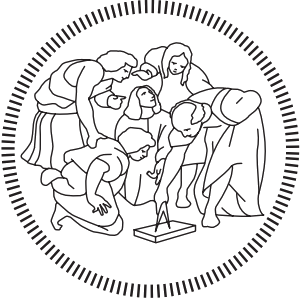
\includegraphics[width=1.5\linewidth]{pictures/newlogo} && \centering \vspace{0.0cm} {\Large POLITECNICO DI MILANO} \newline \small {\large S}CHOOL OF {\large I}NDUSTRIAL AND {\large I}NFORMATION {\large E}NGINEERING
    \end{tabular}
    
  \begin{centering}
    \begin{beamercolorbox}[sep=8pt,center,rounded=true,shadow=true,#1]{title}
      \usebeamerfont{title}\inserttitle\par%
    \end{beamercolorbox}%
  \end{centering}

\vspace{1em}

\begin{tabular}[b]{@{} >{\raggedright\arraybackslash}p{0.5\textwidth} @{}%
   >{\raggedleft\arraybackslash}p{0.5\textwidth} @{}%
  }
Supervisor: Prof. Marcello Restelli &  \\
Co-supervisor: Dott. Alberto Maria Metelli & \\
 \\
& Emanuele Ghelfi, 875550
\end{tabular}

\vspace{1.4em}

\centering
%25/07/2018
20 Dec, 2018

}


\title[Reinforcement Learning in Configurable Environments]{Reinforcement Learning \\ in Configurable Environments: \\ an Information Theoretic approach}
%\subtitle{}

\author[Emanuele Ghelfi]{Emanuele Ghelfi}
\institute[PoliMI]{Politecnico di Milano}
%\logo{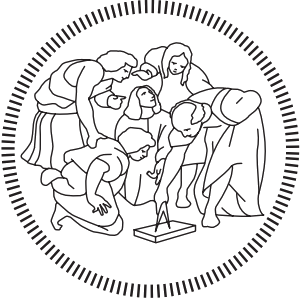
\includegraphics[height=1.0cm]{pictures/newlogo.png}}
 

%\supervisor{Supervisor}{Prof. Marcello Restelli}
\date[20/12/2018]{20 Dicembre 2018}

\supervisor{Prof. Marcello Restelli}

%%%%%% DOCUMENT INIT
\begin{document}

\frame{\titlepage}
\begin{frame}
\frametitle{Contents}
\tableofcontents
\end{frame}

\begin{frame}
	\frametitle{Motivations - Configurable Environments}
	\begin{itemize}
		\item Configure environmental parameters in a principled way.
	\end{itemize}
	\begin{figure}
		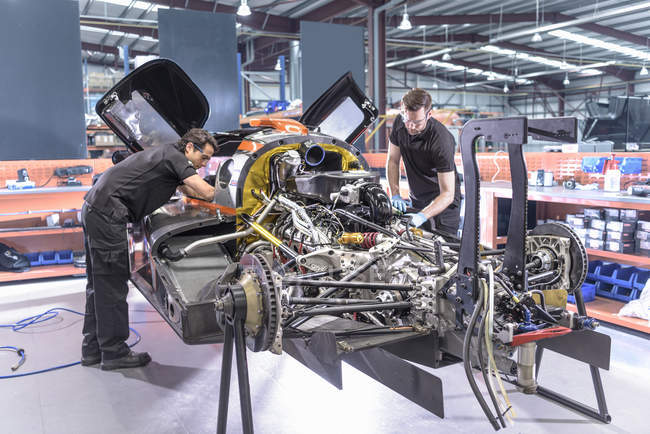
\includegraphics[width=0.46\textwidth]{pictures/conf-env}
		\hspace{1cm}
		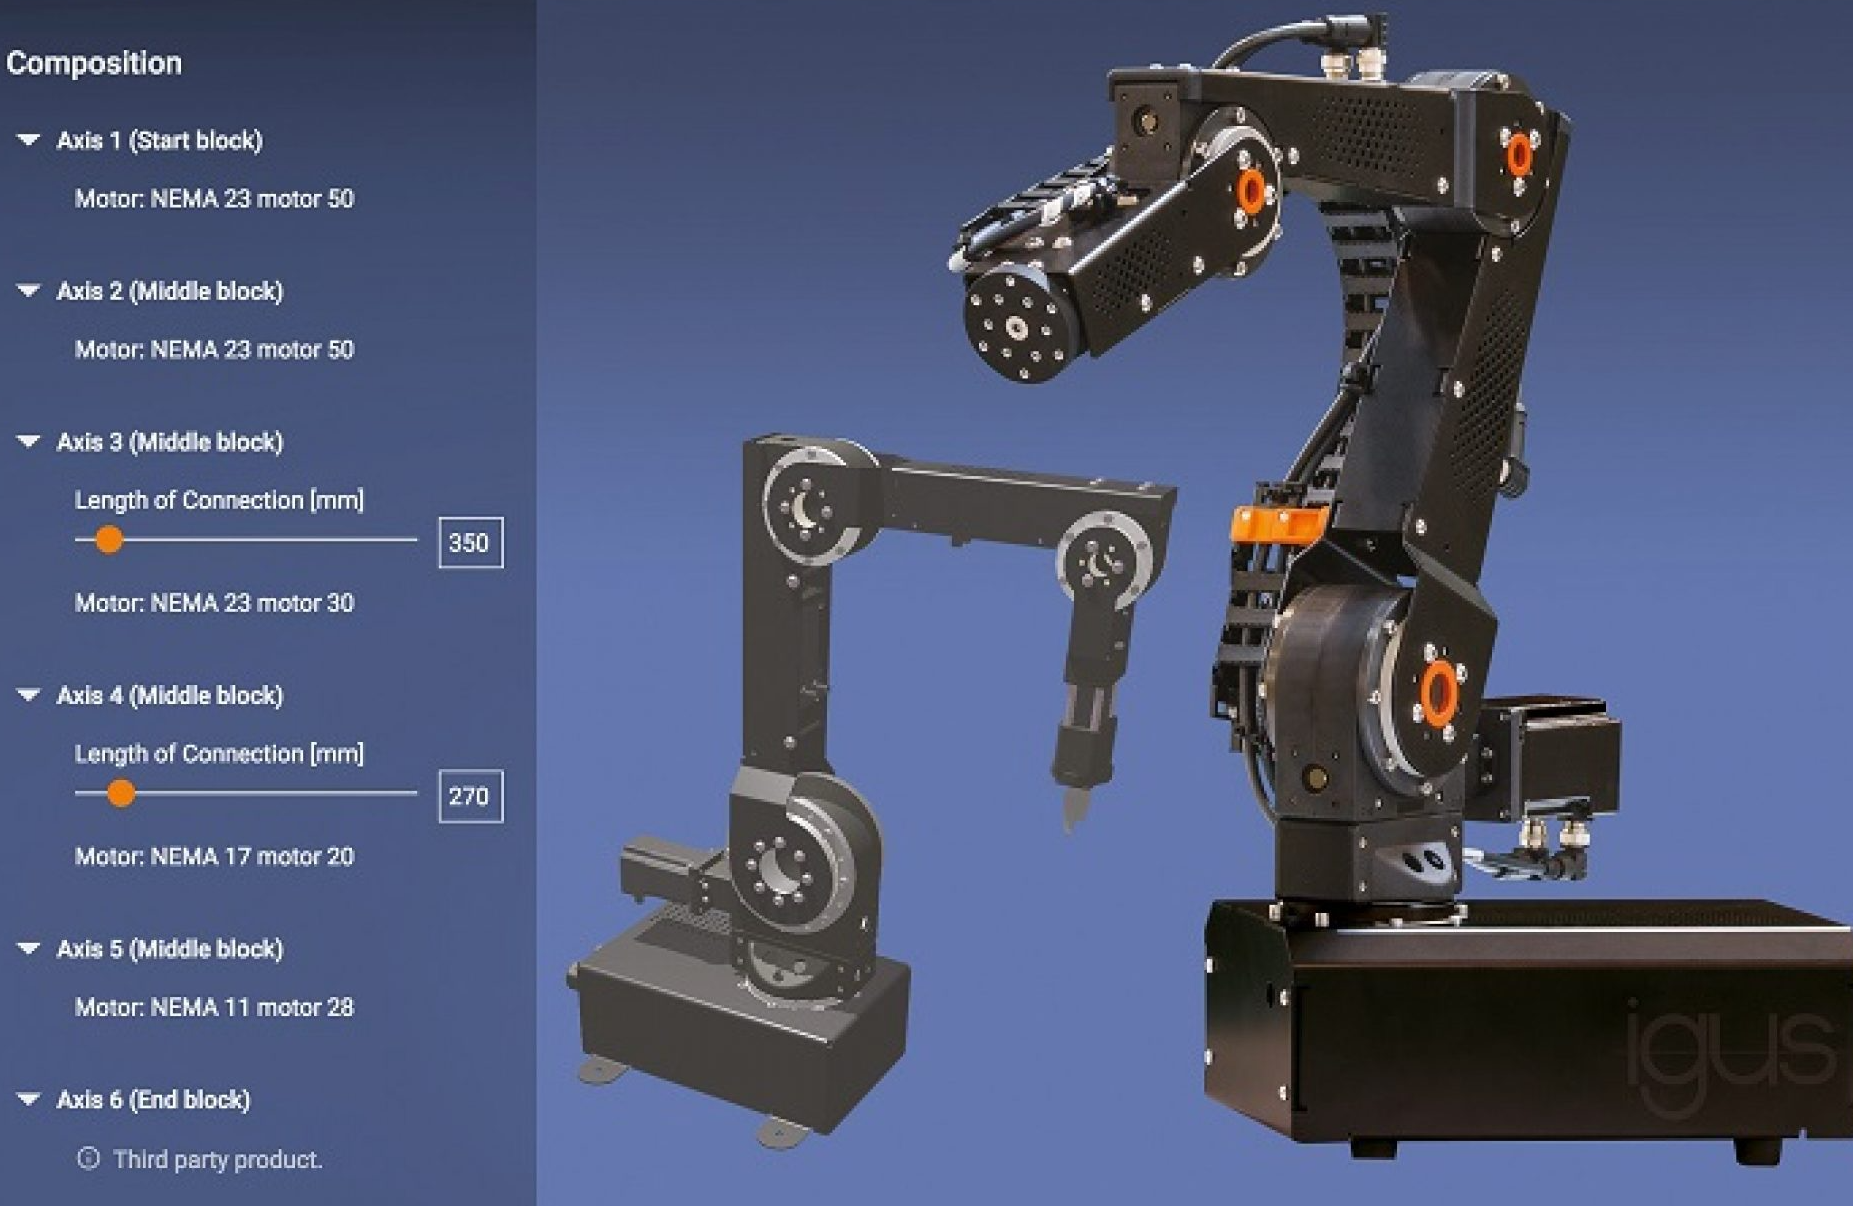
\includegraphics[width=0.46\textwidth]{pictures/conf-env2}
	\end{figure}
\end{frame}

% RL 
\section{Reinforcement Learning}
\begin{frame}
\frametitle{Reinforcement Learning}
Reinforcement Learning \citep{sutton_introduction} considers sequential decision making problems.
\begin{figure}
\centering
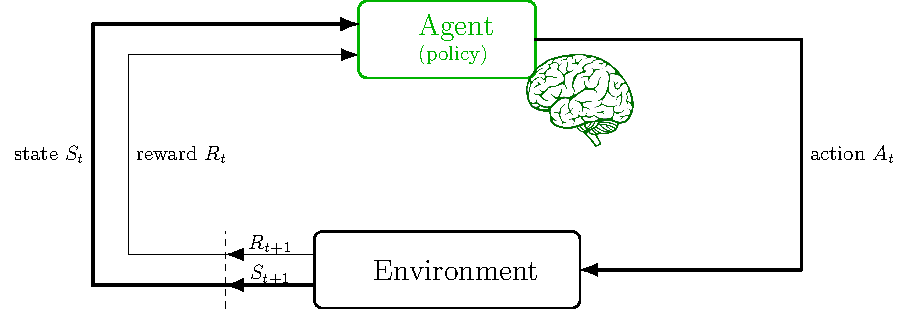
\includegraphics[width=1\textwidth]{pictures/agentenv_v2}
\end{figure}
\end{frame}

%%%%%%%% MDP
%\begin{frame}
%\frametitle{Markov Decision Process}
%\begin{defi}[Markov Decision Process]
%	A Markov Decision Process \citep{Puterman:1994:MDP:528623} (MDP) is a tuple $\langle\mathcal{S}, \mathcal{A}, R, \gamma, P, \mu\rangle$, where:
%\begin{itemize}
%\item $\mathcal{S}$ is  the \textit{state space};
%\item $\mathcal{A}$ is the \textit{action space};
%\item $R : \mathcal{S} \times \mathcal{A} \times \mathcal{S} \rightarrow \mathbb{R}$ is the \textit{reward function};
%\item $\gamma \in [0,1]$ is the \textit{discount factor} for future rewards;
%\item $P: \mathcal{S} \times \mathcal{A} \rightarrow \Delta (\mathcal{S})$ is the \textit{transition function};
%\item $\mu \in \Delta(\mathcal{S}) $ is the initial state distribution.
%\end{itemize}
%\end{defi}
%\end{frame}

%% MDP SOLUTION
\begin{frame}
	\frametitle{Policy Search}
	\begin{defi}[Policy]
	A policy is a function $\pi_{\bm{\theta}}: \mathcal{S} \rightarrow \Delta(\mathcal{A})$ that maps states to probability distributions over actions.
	\end{defi}
	\begin{defi}[Performance]
	The performance of a policy is defined as:
\begin{equation}
	J^\pi = J(\bm{\theta}) = \underset{\begin{subarray}{c}
	a_t \sim \pi(\cdot | s_t) \\
	s_{t+1} \sim P(\cdot | s_t, a_t)
\end{subarray}}{\mathbb{E}} \left[\sum_{t=0}^{H-1} \gamma^t R(s_t,a_t,s_{t+1}) \right] .
\end{equation}
\end{defi}
\begin{defi}[MDP solution]
	An MDP is solved when we find the best performing policy:
\begin{equation}
\bm{\theta}^* \in \arg \max_{\bm{\theta} \in \Theta} J(\bm{\theta}) \, .
\end{equation}
\end{defi}
\end{frame}

%%% Gradient vs information theoretic
%\begin{frame}[t]
%\begin{itemize}
%	\item We consider parameterized policies:
%	\begin{align*}
%		\pi = \pi(\bm{\theta}) \\
%		J^\pi = J(\theta).
%	\end{align*}
%\end{itemize}
%	\begin{figure}
%		\centering
%		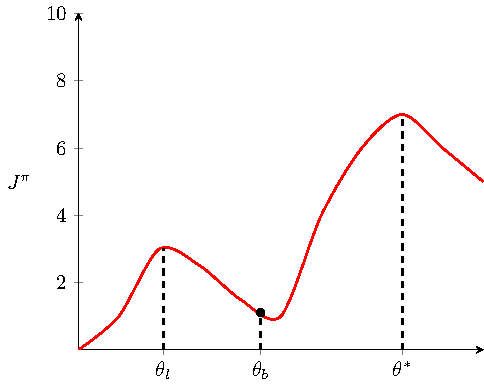
\includegraphics[height=0.7\textheight]{pictures/gradient_methods}
%	\end{figure}
%\end{frame} 

% Policy optimization
%\begin{frame}[t]
%\frametitle{Gradient Methods \citep{gpomdp, reinforce}}
%	Gradient methods optimize performance acting with gradient updates:
%	\begin{equation*}
%		\bm{\theta}^{t+1} = \bm{\theta}^{t} + \lambda \nabla_{\bm{\theta}} J^{\pi} .
%	\end{equation*}
%	\begin{figure}
%		\centering
%		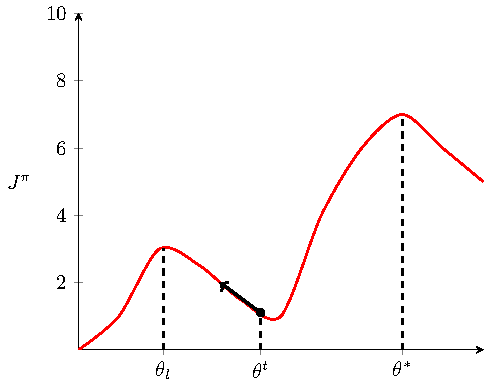
\includegraphics[height=0.66\textheight]{pictures/gradient_methods_arrow}
%	\end{figure}
%\end{frame} 

\begin{frame}[t]
\frametitle{Gradient vs Trust Region}
\begin{columns}[T]
\column{0.5\textwidth}
\centering
	Gradient methods optimize performance acting with gradient updates:
	\begin{equation*}
		\bm{\theta}^{t+1} = \bm{\theta}^{t} + \lambda \nabla_{\bm{\theta}}  J(\bm{\theta}^t) .
	\end{equation*}
	\vspace{-1cm}
	\begin{figure}
		\centering
		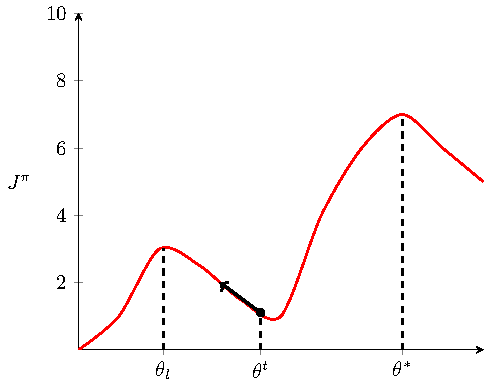
\includegraphics[height=0.55\textheight]{pictures/gradient_methods_arrow}
	\end{figure}
\column{0.5\textwidth}
\centering
\textbf{Trust region} methods perform a constrained optimization:
	\begin{align*}
 		\max_{\bm{\theta}} \; & J(\bm{\theta}) \qquad \text{s.t.} \; \bm{\theta} \in I(\bm{\theta}^t).
 	\end{align*}
 	\vspace{-1cm}
 	\begin{figure}
		\centering
		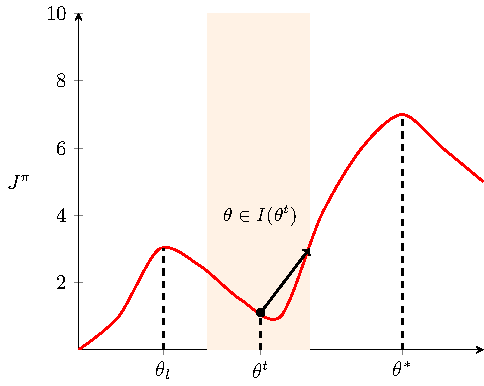
\includegraphics[height=0.55\textheight]{pictures/information_theoretic}
	\end{figure}
	\end{columns}
\end{frame} 


% Policy optimization
%\begin{frame}
%\frametitle{Information theoretic methods}
%	Information theoretic methods rely on the concept of \textbf{trust region}:
%	\begin{align*}
% 		\max_{\bm{\theta}} \; & J(\bm{\theta}) \qquad \text{s.t.} \; \bm{\theta} \in I(\bm{\theta_b}).
% 	\end{align*}
% 	\begin{figure}
%		\centering
%		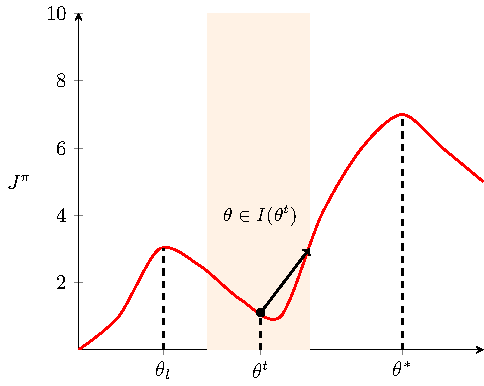
\includegraphics[height=0.66\textheight]{pictures/information_theoretic}
%	\end{figure}
%\end{frame}

%%%% Information theory examples
\begin{frame}
\frametitle{Trust Region methods}
 	\begin{itemize}
 		\item Relative Entropy Policy Search (REPS) \citep{reps}. %uses a constraint on the \textbf{KL--divergence}.
 		\item Trust Region Policy Optimization (TRPO) \citep{trpo}. %uses a \textbf{penalty} instead of a constraint.
 		\item Proximal Policy Optimization (PPO) \citep{ppo}. %uses a \textbf{clipped objective}.
 		\item Policy Optimization via Importance Sampling (POIS) \citep{metellipolicy2018}. %uses as penalization the \textbf{Rényi divergence}.
 	\end{itemize}
\end{frame} 

\section{Configurable MDP}
% CMDP
\begin{frame}
\frametitle{Configurable MDP}
A \textcolor{red}{Configurable} Markov Decision Process \citep{cmdp} (\textbf{CMDP}) is an MDP extension.
\begin{figure}
\centering
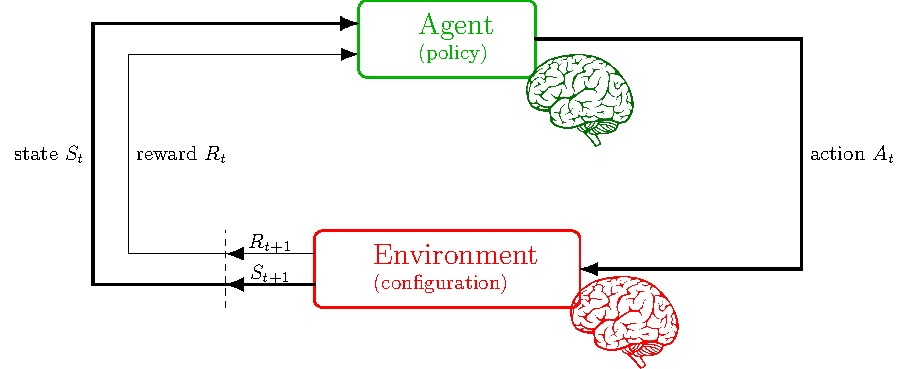
\includegraphics[width=1\textwidth]{pictures/agentenvsup_v2}
\end{figure}
\end{frame}
% More about RL
%\begin{frame}
%\frametitle{Configurable MDP}
%Rationale: \textbf{configure} the \textbf{environment} and the \textbf{policy} to optimize the performance. \hfill
%\begin{defi}[Configurable Markov Decision Process]
%A Configurable Markov Decision Process is a tuple $\mathcal{CM}= \langle \mathcal{S}, \mathcal{A}, R, \mu, \gamma, \mathcal{P}, \Pi\rangle$, where $\langle \mathcal{S}, \mathcal{A}, R, \mu, \gamma \rangle$ is an MDP without the transition model, $\mathcal{P}$ is the \textbf{model space} and $\Pi$ is the \textbf{policy space}.
% \end{defi}
%\end{frame}

% More about CMDP
\begin{frame}
\frametitle{Configurable MDP}
\begin{defi}[CMDP performance]
The performance of a \textcolor{red}{model}-\textcolor{green!80!black}{policy} pair is:
\begin{equation}
	J^{\textcolor{red}{P},\textcolor{green!80!black}{\pi}} = J(\textcolor{red}{\bm{\omega}},\textcolor{green!80!black}{\bm{\theta}}) = \underset{\begin{subarray}{c}
	a_t \sim \pi(\cdot | s_t) \\
	s_{t+1} \sim P(\cdot | s_t, a_t)
\end{subarray}}{\mathbb{E}} \left[\sum_{t=0}^{H-1} \gamma^t R(s_t,a_t,s_{t+1}) \right] .
\end{equation}
\end{defi}
	\begin{defi}[CMDP Solution]
 	The CMDP solution is the \textcolor{red}{model}-\textcolor{green!80!black}{policy} pair maximizing the performance:
\begin{equation}
	\textcolor{red}{\bm{\omega}^*}, \textcolor{green!80!black}{\bm{\theta}^*} \in \underset{\bm{\omega} \in \Omega, \bm{\theta} \in \Theta}{\arg \max} J(\bm{\omega},\bm{\theta})  \, .
\end{equation}
 \end{defi}
\end{frame}

% SPMI
\begin{frame}[t]
\frametitle{State of the Art}
Safe Policy Model Iteration \citep{cmdp}:
\begin{itemize}
	\item Safe Approach \citep{pmlr-v28-pirotta13} for solving CMDPs:
	 \begin{equation}
	\underbrace{J^{P', \pi'} - J^{P, \pi}}_{\text{Performance improvement}} \geq B(P',\pi') = \underbrace{\frac{\mathds{A}_{P,\pi,\mu}^{P',\pi}+\mathds{A}_{P,\pi, \mu}^{P,\pi'}}{1-\gamma}}_{\text{Advantage term}}-\underbrace{\frac{\gamma\Delta q^{P,\pi}D}{2 (1 -\gamma)^2}}_{\text{Dissimilarity Penalization}} \, .
	\label{eq:spmi-lower}
\end{equation}
\end{itemize}
Limitations:
\begin{itemize}
	\item \textbf{Finite} state-actions space.
	\item \textbf{Full knowledge} of the environment dynamics.
	\item High sample complexity.
\end{itemize}
\end{frame}

\section{Contribution - Relative Entropy Model Policy Search}
% REMPS
\begin{frame}[t]
\frametitle{Relative Entropy Model Policy Search}
We present \textbf{REMPS}, a novel algorithm for \textbf{CMDP}s:
\vspace{1em}
\begin{itemize}
	\item \textbf{Information Theoretic} approach.
	\item \textbf{Optimization} and \textbf{Projection}.
	\item \textbf{Approximated} models.
	\item \textbf{Continous} state and action spaces.
\end{itemize}
	We optimize the \textbf{Average Reward}:
	$$
J^{P,\pi} = \underset{H \rightarrow + \infty}{\lim \inf} \underset{\begin{subarray}{c}
	a_t \sim \pi(\cdot | s_t) \\
	s_{t+1} \sim P(\cdot | s_t, a_t)
\end{subarray}}{\mathbb{E}} \left[ \frac{1}{H} \sum_{t=0}^{H-1} R(s_t,a_t,s_{t+1}) \right] .
$$

\end{frame}

\begin{frame}
\frametitle{REMPS - Optimization}
\begin{itemize}
	\item  We define the following constrained optimization problem:
\end{itemize}
\begin{columns}[T]
\column{0.5\textwidth}
\centering
\textbf{Primal}
\begin{align*}
	\max_{d} & \; \mathbb{E}_{d} [R(s,a,s')] \\
	\text{subject to:} &\\
	& D_{KL}(d || d^{P,\pi}) 
	%=  \sas d_{\mu,\gamma}^{P,\pi}(s,a,s') \log \frac{d_{\mu,\gamma}^{P,\pi}(s,a,s')}{\widetilde{d}_{\mu,\gamma}^{P,\pi}(s,a,s')} ds da ds'
	\leq \epsilon \\
	& \mathbb{E}_{d} [1] = 1 \, .
\end{align*}
\column{0.5\textwidth}
\centering
\textbf{Dual}
\begin{align*}
	\min_{\eta} & \; \eta \log \left( \mathbb{E}_{d^{P,\pi}} \left[ e^{\left(\epsilon + \frac{R(s,a,s')}{\eta} \right)}\right] \right) \\
	\text{subject to:} &\\
	& \eta \geq 0.	
	\label{eq:remps-dual}
\end{align*}
\end{columns}
\begin{itemize}
\item $d^{P,\pi}$: \textbf{sampling distribution}.
\item $\epsilon$: \textbf{Trust Region}.
\item $d$: stationary distribution over state, action and next-state.
\end{itemize}
\end{frame}


\begin{frame}
\frametitle{REMPS - Optimization}
\hspace{0.45\textwidth} \textbf{Primal}
\hfsetfillcolor{blue!10}
\hfsetbordercolor{blue}
\begin{align*}
\only<1>{\tikzmarkin{a}(0.2,-0.5)(-0.2,0.65)}
	\max_{d} & \; \mathbb{E}_{d} [R(s,a,s')] \only<1>{\qquad \text{Objective Function} \tikzmarkend{a}}\\
	\text{subject to:} & \notag\\
	& \only<2>{\tikzmarkin{b}(0.2,-0.2)(-0.2,0.45)} D_{KL}(d || d^{P,\pi})
	%=  \sas d_{\mu,\gamma}^{P,\pi}(s,a,s') \log \frac{d_{\mu,\gamma}^{P,\pi}(s,a,s')}{\widetilde{d}_{\mu,\gamma}^{P,\pi}(s,a,s')} ds da ds'
	\leq \epsilon \only<2>{\qquad \text{Trust Region}\tikzmarkend{b}} \\
	& \only<3>{\tikzmarkin{c}(0.2,-0.2)(-0.2,0.45)} \mathbb{E}_{d} [1] = 1 \, . \only<3>{\qquad \text{$d$ is well formed}  \tikzmarkend{c}}
\end{align*}
\begin{itemize}
\item $d^{P,\pi}$: sampling distribution.
\item $\epsilon$: \textbf{Trust Region}.
\item $d$: stationary distribution.
\end{itemize}
\end{frame}

\begin{frame}
\frametitle{REMPS - Optimization Solution}
\begin{thr}[REMPS solution]
The solution of the REMPS problem is:
\begin{equation}
	d(s,a,s') = \frac{d^{P,\pi}(s,a,s') \exp \left(\frac{R(s,a,s')}{\eta} \right)}{\sas d^{P,\pi}(s,a,s') \exp \left( \frac{R(s,a,s')}{\eta} \right) \mathrm{d}s \mathrm{d}a \mathrm{d}s' } \,
\end{equation}
where $\eta$ is the minimizer of the dual problem.
\end{thr}
\begin{itemize}
	\item Probability of $(s,a,s')$ weighted exponentially with the reward.
\end{itemize}
\end{frame}

%\begin{frame}
%\frametitle{REMPS - Optimization Solution}
%\begin{cor}
%	The REMPS solution is induced by the optimal model and policy:
%\begin{align}
%	\pi'(a | s) &= \frac{\pi(a | s) \int_\mathcal{S} P(s' | s,a) \exp \left( \epsilon + \frac{R(s,a,s')}{\eta} \right) \mathrm{d}s'}{\int_\mathcal{A} \pi(a | s) \int_\mathcal{S} P(s' | s,a) \exp \left( \epsilon + \frac{R(s,a,s')}{\eta} \right) \mathrm{d}s' \mathrm{d}a} \\
%	P'(s' | a, s) & = \frac{P(s' | s,a) \exp \left( \epsilon + \frac{R(s,a,s')}{\eta} \right)}{\int_\mathcal{S} P(s' | s,a) \exp \left( \epsilon + \frac{R(s,a,s')}{\eta} \right) \mathrm{d}s'}  \, .
%\end{align}
%\end{cor}
%\end{frame}

%\begin{frame}
%\frametitle{REMPS - Projection}
%\begin{itemize}
%	\item The solution of the optimization phase lies on the space of \textbf{all} stationary distributions.
%	\item The solution might be \textbf{not} representable.  
%	\item We need to find a \textbf{representable} distribution.
%	\item We propose a \textbf{Moment Projection}, as in \citep{danielhierarchicalnodate} to obtain a feasible distribution.
%\end{itemize}
%\end{frame}

\begin{frame}
	\frametitle{REMPS - Projection}
	\begin{figure}
	\only<1>{
		\includegraphics[height=0.8\textheight]{pictures/information_projection_1}
		}
		\only<2>{
		\includegraphics[height=0.8\textheight]{pictures/information_projection_2}
		}
		\only<3>{
		\includegraphics[height=0.8\textheight]{pictures/information_projection_3}
		}
		\only<4>{
		\includegraphics[height=0.8\textheight]{pictures/information_projection_4}
		}
		\only<5>{
		\includegraphics[height=0.8\textheight]{pictures/information_projection_5}
		}
	\end{figure}
\end{frame}

\begin{frame}
	\frametitle{REMPS - Projection}
	\begin{columns}[T]
\column{0.3\textwidth}
\centering
\textbf{$d$-Projection}
\vspace{0.3cm}
\begin{itemize}
\item Discrete state-action spaces.
\item $\underset{\bm{\theta} \in \Theta, \bm{\omega} \in \Omega}{\arg \min} D_{KL} \left(d \| d^{\bm{\omega}, \bm{\theta}}\right)$.
\end{itemize}
\column{0.3\textwidth}
\centering
\textbf{State-Kernel Projection}
\vspace{0.3cm}
\begin{itemize}
\item Discrete action spaces.
\item $\underset{\bm{\theta} \in \Theta, \bm{\omega} \in \Omega}{\arg \min} \mathbb{D}_{KL}(P^{\pi} \| P_{\bm{\omega}}^{\pi_{\bm{\theta}}})$.
\end{itemize}
\column{0.3\textwidth}
\centering
\textbf{Independent Projection}
\vspace{0.3cm}
\begin{itemize}
\item Continuous state action spaces.
\item $\underset{\bm{\theta} \in \Theta}{\arg \min} \mathbb{D}_{KL} (\pi' \| \pi_{\bm{\theta}})$.
\item $\underset{\bm{\omega} \in \Omega}{\arg \min} \mathbb{D}_{KL} (P' \| P_{\bm{\omega}})$.
\end{itemize}
\end{columns}
\end{frame}

\begin{frame}
	\frametitle{Algorithm}
	\begin{algorithm}[H]
  \caption{Relative Entropy Model Policy Search}
  \begin{algorithmic}[1]
  \For{t = 0,1,... until convergence}
  \State Collect samples from $\pi_{\bm{\theta}_t}, P_{\bm{\omega}_t}$
  \State Obtain $\eta^*$, the minimizer of the dual problem. \Comment{\textbf{Optimization}}
  \State Project $d$ according to the projection strategy. \Comment{\textbf{Projection}}
  \begin{description}
  	\item[a.] $d$-Projection;
  	\item[b.] State-Kernel Projection;
    \item[c.] Independent Projection.
\end{description}
  \State Update Policy.
  \State Update Model.
  \EndFor \\
  \Return{Policy-Model Pair $\left( \pi_{\bm{\theta}_t}, P_{\bm{\omega}_t} \right)$
  } 	
  \end{algorithmic}
\end{algorithm}
\end{frame}

\section{Finite--Sample Analysis}
\begin{frame}
	\frametitle{Finite--Sample Analysis}
	How much can differ the ideal performance from the approximated one?
	\begin{itemize}
		\item $d$ solution of Optimization with $\infty$ samples.
		\item $\widetilde{d}$ solution of Optimization with $N$ samples.
		\item $\widetilde{d}'$ solution of Optimization and Projection with $N$ samples.
	\end{itemize}
	\begin{align}
	J_d - J_{\widetilde{d}'} =& \textcolor{blue}{\underbrace{J_d - J_{\widetilde{d}}}_{\text{OPT}}} + \textcolor{violet}{\underbrace{J_{\widetilde{d}}- J_{\widetilde{d}'}}_{\mathrm{PROJ}}}.
	\end{align}
\end{frame}
\begin{frame}
	\frametitle{Finite--Sample Analysis}
	How much can differ the ideal performance from the approximated one?
	\begin{align}
	J_d - J_{\widetilde{d}'} \leq & \; \textcolor{blue}{r_{\max} \psi(N) \sqrt{\frac{8v \log\frac{2eN}{v} + 8 \log \frac{8}{\delta}}{N}}} \\
	& + \textcolor{violet}{r_{\max} \phi \sqrt[4]{\frac{8v \log\frac{2eN}{v} + 8 \log \frac{8}{\delta}}{N}}} \\
		& + \textcolor{violet}{\sqrt{2} r_{\max} \sup_{d \in \mathcal{D}_{d^{P,\pi}}}  \inf_{\overline{d} \in \mathcal{D}_{\mathcal{P},\Pi}} \sqrt{D_{KL}( d \| \overline{d})}}.
	\end{align}
\end{frame}

\section{Experiments}
\begin{frame}
	\frametitle{Experimental Results - Chain}
	\textbf{Motivations}: \begin{itemize}
 \item Visualize the behaviour of \textbf{REMPS};
 \item Overcoming local minima;
 \item Configure transition function.
 \end{itemize}
 \vspace{-2.3cm}
	\begin{columns}[T]
	\column{0.5\textwidth}
	\centering
	\vspace{2cm}
	\begin{figure}
		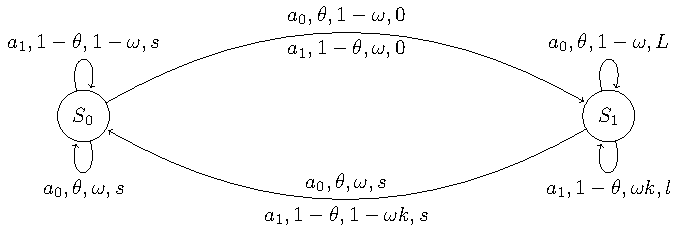
\includegraphics[width=1.2\textwidth]{pictures/chain}
	\end{figure}
	\column{0.5\textwidth}
	\centering
	\begin{figure}
		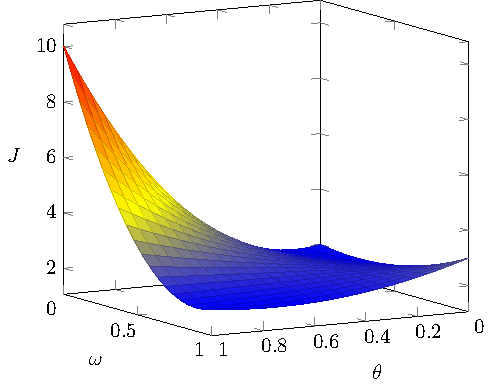
\includegraphics[height=0.42\textheight]{plots/chain/plot_chain_surface} \\
		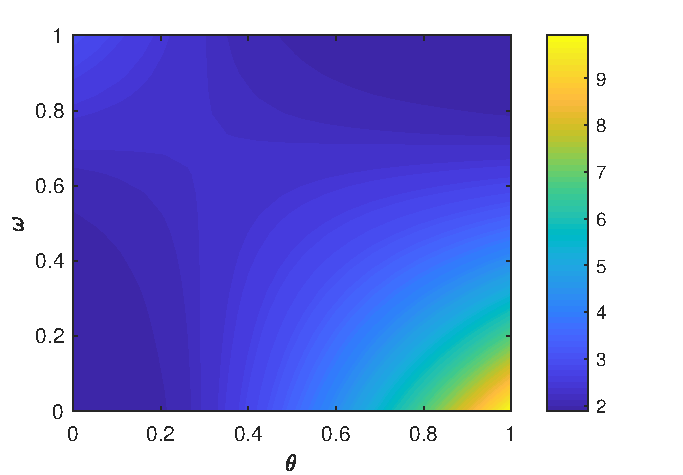
\includegraphics[height=0.42\textheight]{plots/chain/plot_chain_colormap}
	\end{figure}
	\end{columns}
\end{frame}

\begin{frame}
	\frametitle{Experimental Results - Chain}
	\begin{figure}
	\only<1>{
		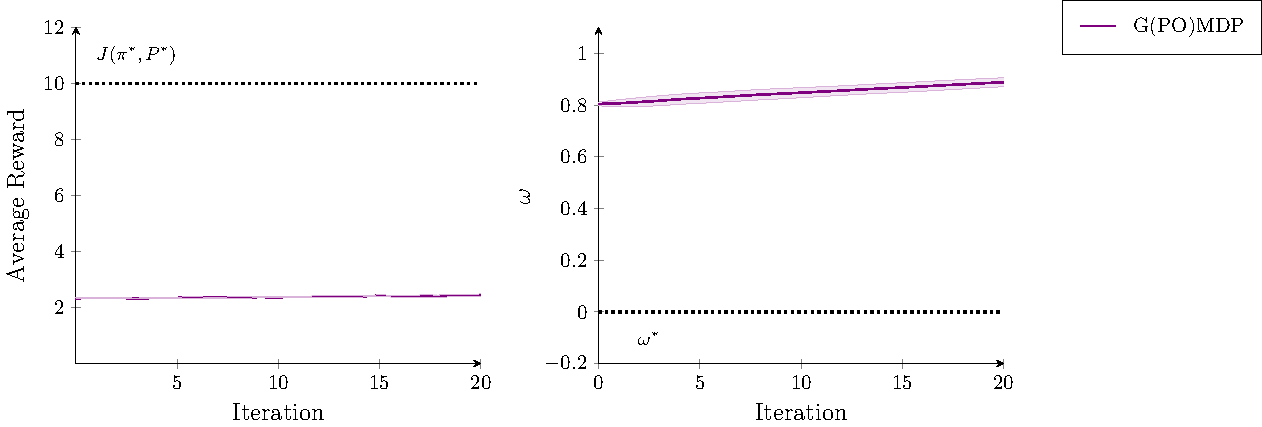
\includegraphics[width=1\textwidth]{plots/chain/plot_chain_all_small_1}}
		\only<2>{
		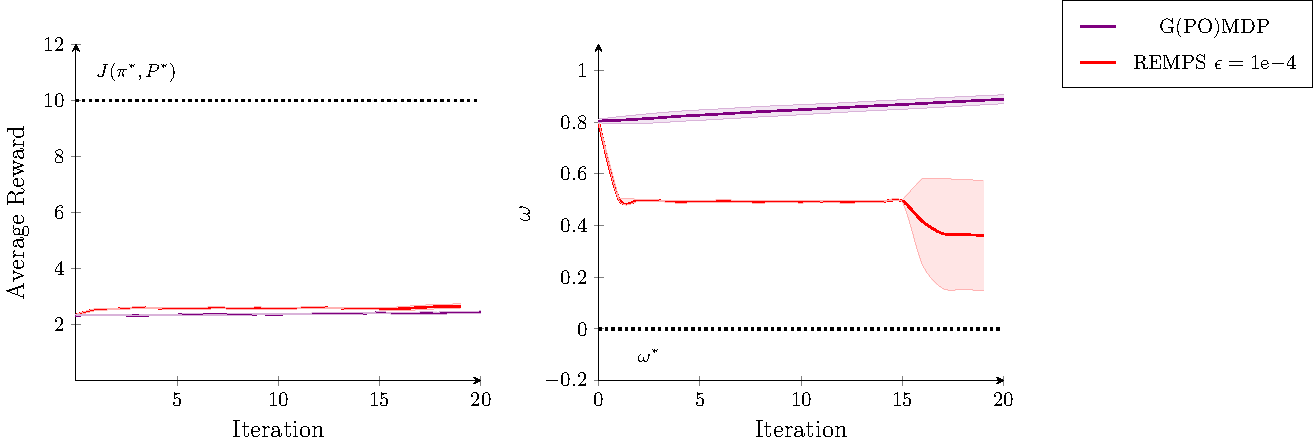
\includegraphics[width=1\textwidth]{plots/chain/plot_chain_all_small_2}}
		\only<3>{
		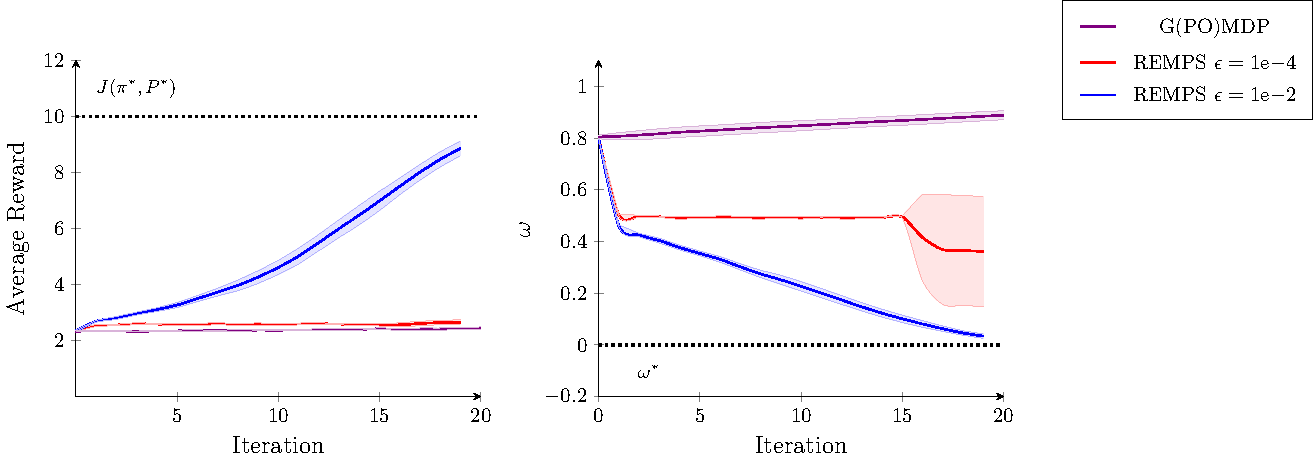
\includegraphics[width=1\textwidth]{plots/chain/plot_chain_all_small_3}}
		\only<4>{
		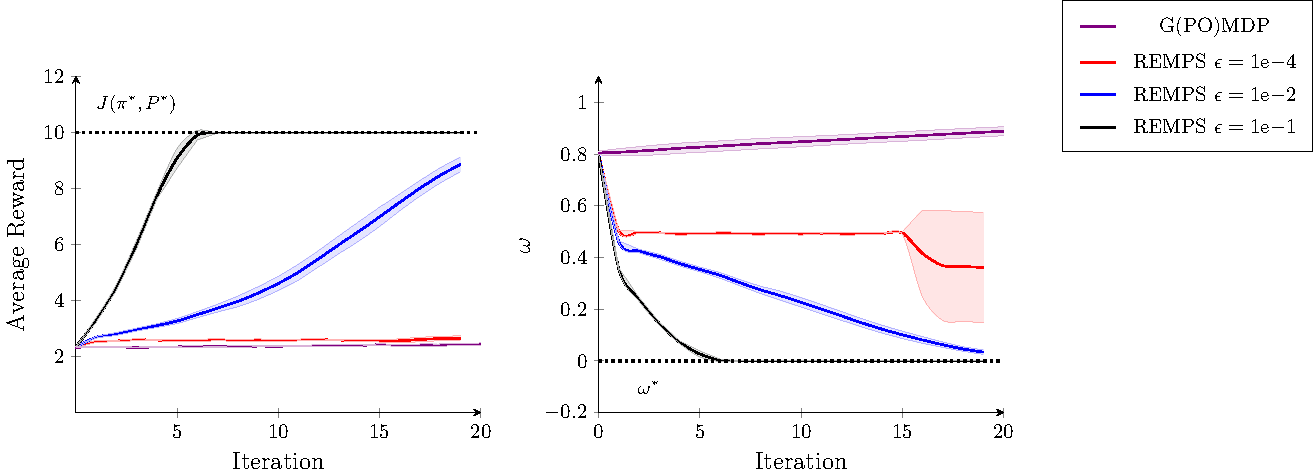
\includegraphics[width=1\textwidth]{plots/chain/plot_chain_all_small_4}}
		\only<5>{
		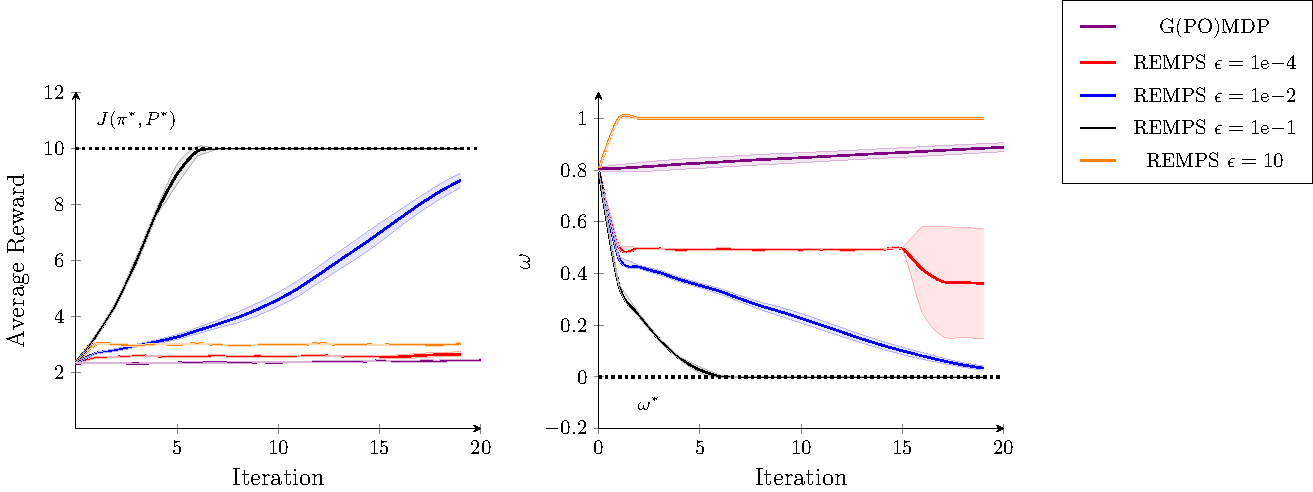
\includegraphics[width=1\textwidth]{plots/chain/plot_chain_all_small_5}}
	\end{figure}
\end{frame}

\begin{frame}
	\frametitle{Experimental Results - Cartpole}
\begin{itemize}
 	\item Standard RL benchmark;
 	\item Configure cart \textbf{acceleration};
 	\item Approximated model.
 	\end{itemize}
Minimize acceleration balancing the pole: \newline
$
R(s,a,s') = 10 - \frac{\omega^2}{20} - 20 \cdot (1 - \cos(\gamma)) .
 $
 	\vspace{-3cm}
	\begin{figure}
	\hspace{2cm}
		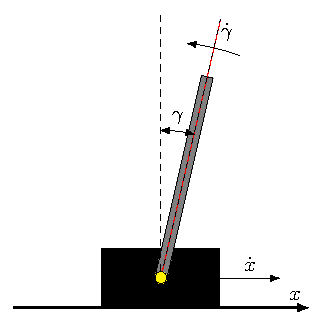
\includegraphics[height=0.7\textheight]{plots/cartpole/cartpole_env}
	\end{figure}
\end{frame}

\begin{frame}
	\frametitle{Experimental Results - Cartpole}
	\hspace{2cm} \textbf{Ideal Model} \hspace{3cm} \textbf{Approximated Model}
	\vspace{-1cm}
	\begin{figure}
		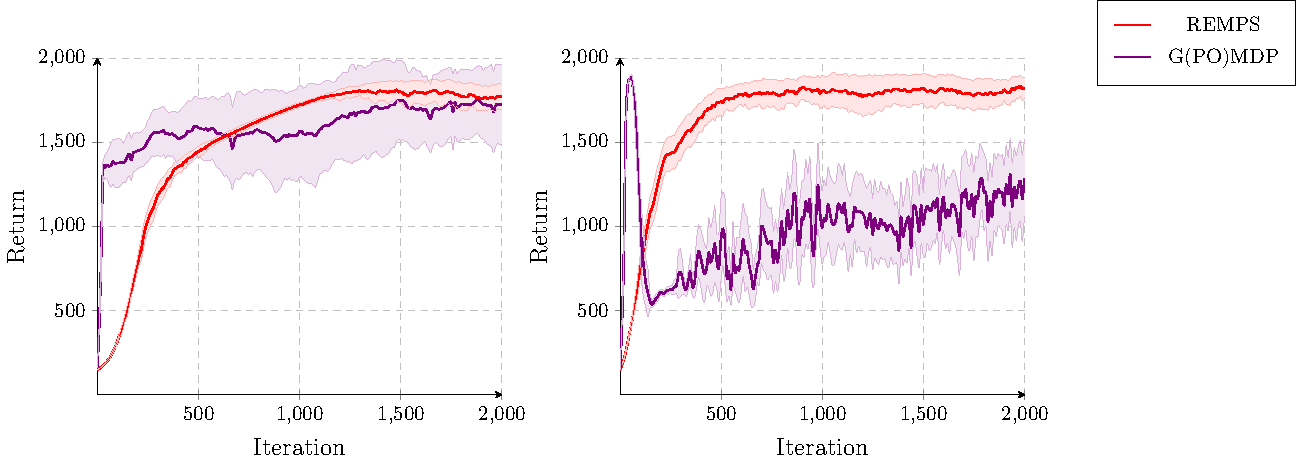
\includegraphics[width=1\textwidth]{plots/cartpole/plot_cartpole_experiment_small}
	\end{figure}
\end{frame}

\begin{frame}
	\frametitle{Experimental Results - TORCS}
	TORCS: Car Racing simulation \citep{TORCS, torcs-1}. \newline
	\vspace{-0.5cm}
	\begin{itemize}
		\item Autonomous driving and \textbf{Configuration}.
		\item \textbf{Continuous Control}.
		\item Approximated model.
		\item We configure the \textbf{rear wing} and the \textbf{brake system}.
	\end{itemize}
	\begin{figure}
	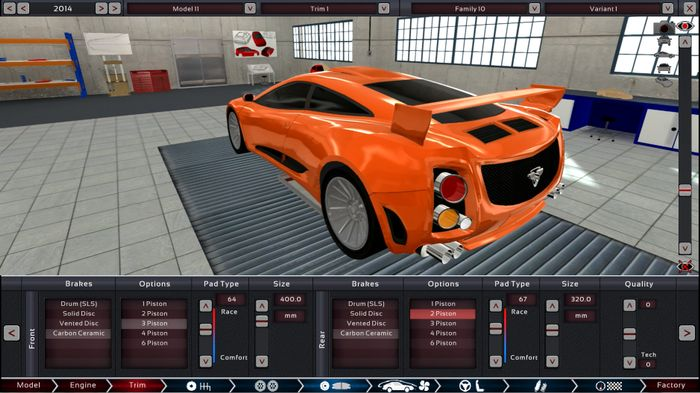
\includegraphics[width=0.4\textwidth]{pictures/car-conf}
	\hspace{1cm}
		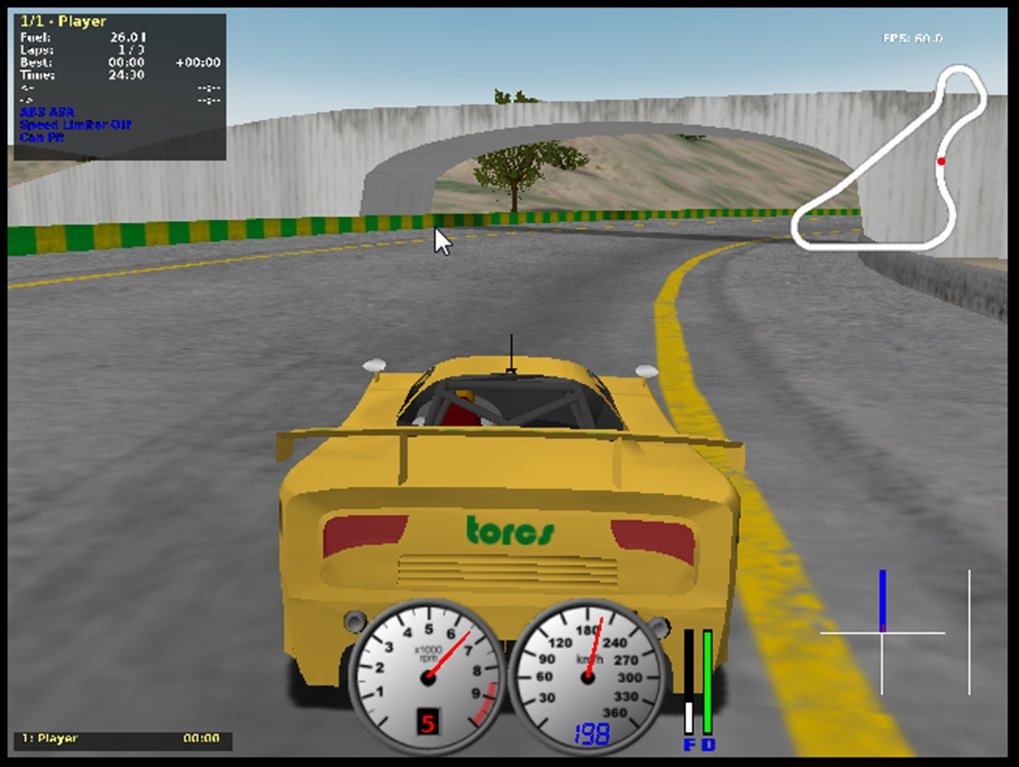
\includegraphics[width=0.3\textwidth]{pictures/torcs_image}
	\end{figure}
\end{frame}

\begin{frame}
	\frametitle{Experimental Results - TORCS}
	\begin{figure}
		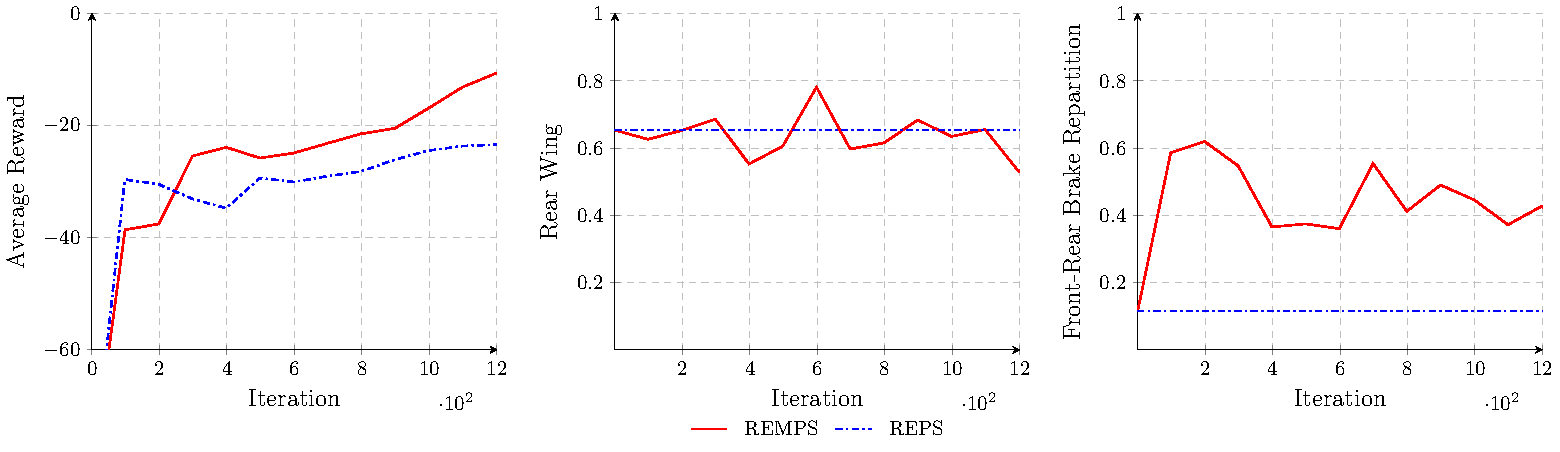
\includegraphics[width=1\textwidth]{plots/torcs/plot_torcs}
	\end{figure}
\end{frame}

\begin{frame}[t]
\frametitle{Conclusions}
\begin{itemize}
\item Contributions:
\begin{itemize}
	\item \textbf{REMPS} able to solve the model-policy learning problem.
	\item \textbf{Finite-sample} analysis.
	\item \textbf{Experimental} evaluation.
\end{itemize}
\item Future research directions:
\begin{itemize}
	\item Adaptive KL-constraint.
	\item Other divergences.
	\item Finite-Time Analysis.
\end{itemize}
\item Plan to submit at \textbf{ICML} 2019.
\end{itemize}
\end{frame}

\begin{frame}{Conclusions}
\centering
\LARGE Thank you for your attention\\
\vspace{2cm}
Questions?
\end{frame}

\begin{frame}[allowframebreaks]
        \frametitle{Bibliography}
        \bibliographystyle{mydinat}
        \bibliography{bibl_tesi}
\end{frame}

\begin{frame}
	\frametitle{$d$-projection}
	Projection of the stationary state distribution:
	\begin{align*}
	& \widehat{\bm{\theta}}, \widehat{\bm{\omega}} = \arg \min_{\bm{\theta} \in \Theta, \bm{\omega} \in \Omega} D_{KL} \left(d(s,a,s') \| d^{\bm{\omega}, \bm{\theta}}(s,a,s')\right)  \\
    & s.t. \; d^{\bm{\omega}, \bm{\theta}}(s) =\int_{\mathcal{S}} \int_{\bm{A}}d^{\bm{\omega}, \bm{\theta}}(s') \pi_{\bm{\theta}}(a|s') P_{\bm{\omega}}(s'|s,a) \mathrm{d}a \mathrm{d}s'.
\end{align*}
\end{frame}

\begin{frame}
	\frametitle{Projection of the State Kernel}
	Projection of the state kernel:
	\begin{align*}
	\widehat{\bm{\theta}}, \widehat{\bm{\omega}} & = \arg \min_{\bm{\theta} \in \Theta, \bm{\omega} \in \Omega} \int_{\mathcal{S}} d(s) D_{KL} (P^{\pi}(\cdot|s) \| P_{\bm{\omega}}^{\pi_{\bm{\theta}}}(\cdot|s)) \mathrm{d}s \\
    & = \arg \max_{\bm{\theta} \in \Theta, \bm{\omega} \in \Omega} \int_{\mathcal{S}} d(s) \int_{\mathcal{S}} P^{\pi}(s'|s) \log P_{\bm{\omega}}^{\pi_{\bm{\theta}}}(s'|s) \mathrm{d}s' \mathrm{d}s \\
    & = \arg \max_{\bm{\theta} \in \Theta, \bm{\omega} \in \Omega} \int_{\mathcal{S}} d(s) \int_{\mathcal{S}} \int_{\mathcal{A}} \pi'(a|s)P'(s'|s, a) \log P_{\bm{\omega}}^{\pi_{\bm{\theta}}}(s'|s) \mathrm{d}s' \mathrm{d}s \\
    & = \arg \max_{\bm{\theta} \in \Theta, \bm{\omega} \in \Omega} \int_{\mathcal{S}}\int_{\mathcal{A}}\int_{\mathcal{S}} d(s,a,s') \log \int_{\mathcal{A}} P_{\bm{\omega}}(s'|s,a') \pi_{\bm{\theta}}(a'|s) \mathrm{d}a' \mathrm{d}s \mathrm{d}a \mathrm{d}s'
\end{align*}
\end{frame}

\begin{frame}
	\frametitle{Independent Projection}
	Independent Projection of policy and model:
	\begin{align}
	\widehat{\bm{\theta}} & = \arg \min_{\bm{\theta} \in \Theta} \int_{\mathcal{S}} d(s) D_{KL} (\pi'(\cdot|s) \| \pi_{\bm{\theta}} (\cdot|s)) \mathrm{d}s = \\
    & = \arg \min_{\bm{\theta} \in \Theta} \int_{\mathcal{S}} d(s) \int_{\mathcal{A}} \pi'(a|s) \log \frac{\pi(a|s)}{\pi_{\bm{\theta}} (a|s)} \mathrm{d}a \mathrm{d}s = \\
    & = \arg \min_{\bm{\theta} \in \Theta} \int_{\mathcal{S}} \int_{\mathcal{A}}  \int_{\mathcal{S}}  d(s,a,s') \log \frac{\pi'(a|s)}{\pi_{\bm{\theta}} (a|s)} \mathrm{d}s \mathrm{d}a \mathrm{d}s' = \\
    & = \arg \max_{\bm{\theta} \in \Theta} \int_{\mathcal{S}} \int_{\mathcal{A}}  \int_{\mathcal{S}} d(s,a,s') \log \pi_{\bm{\theta}} (a|s) \mathrm{d}s \mathrm{d}a \mathrm{d}s',
\end{align}
	
\end{frame}

\begin{frame}
\frametitle{Projection}

	\begin{thr}[Joint bound]
Let us denote with $d^{P,\pi}$ the stationary distribution induced by the model $P$ and policy $\pi$ and $d^{P',\pi'}$ the stationary distribution induced by the model $P'$ and policy $\pi'$. Let us assume that the reward is uniformly bounded, that is for $s, s' \in \mathcal{S}$, $a \in \mathcal{A}$ it holds that $|R(s,a,s')| < R_{\max}$. The norm of the difference of performance can be upper bounded as:
\begin{equation}
	|J^{P,\pi} - J^{P',\pi'}| \leq R_{\max} \sqrt{2 D_{KL} (d^{P,\pi} \| d^{P',\pi'})}.
\end{equation}
\end{thr}
\end{frame}

\begin{frame}
\frametitle{Projection}
\begin{thr}[Disjoint bound]
Let us denote with $d^{P,\pi}$ the stationary distribution induced by the model $P$ and policy $\pi$, $d^{P',\pi'}$ the stationary distribution induced by the model $P'$ and policy $\pi'$. Let us assume that the reward is uniformly bounded, that is for $s, s' \in \mathcal{S}$, $a \in \mathcal{A}$ it holds that $|R(s,a,s')| < R_{\max}$. If $(P',\pi')$ admits group invertible state kernel $P'^{\pi'}$ the norm of the difference of performance can be upper bounded as:
\begin{equation}
	|J^{P,\pi} - J^{P',\pi'}| \le R_{\max} \, c_1 \mathbb{E}_{s,a \sim d^{P,\pi}} \left[ \sqrt{2D_{KL}(\pi'\|\pi)} + \sqrt{2D_{KL}(P'\|P)} \right],
\end{equation}
where $c_1 = 1 + ||A'^{\#}||_{\infty}$ and $A'^{\#}$ is the group inverse of the state kernel $P'^{\pi'}$.
\end{thr}
\end{frame}

\begin{frame}
\frametitle{G(PO)MDP - Model extension}
	$$
J^{P,\pi} = \int p_{\boldsymbol{\theta},\boldsymbol{\omega}}(\tau)G(\tau) \mathrm{d}\tau
$$
\begin{align}
	\nabla_{\boldsymbol{\omega}}J^{P,\pi} &= \int p_{\boldsymbol{\theta},\boldsymbol{\omega}}(\tau) \nabla_{\boldsymbol{\omega}}\log p(\tau) G(\tau) \mathrm{d}\tau \\
	&= \int p_{\boldsymbol{\theta},\boldsymbol{\omega}}(\tau) \left(\sum_{k=0}^{H} \log P_{\boldsymbol{\omega}}(s_{k+1} | s_k, a_k)  \right) G(\tau)
\end{align}
\begin{equation}
\widehat{\nabla_{\boldsymbol{\omega}} J^{P\pi}}_{G(PO)MDP} = \langle \sum_{l=0}^H \left( \sum_{k=l}^H \nabla_{\bm{\omega}} \log P_{\boldsymbol{\omega}}(s_{k+1} | s_k, a_k) \right) \left( \gamma^l R(s_l,a_l, s_{l+1}) \right) \rangle_N \,
\end{equation}

\end{frame}

\end{document}
